\pdfinfo{%
  /Title    ()
  /Author   ()
  /Creator  ()
  /Producer ()
  /Subject  ()
  /Keywords ()
}

\section{Newseinträge löschen}
Newseinträge werden vom Administrator verfasst und verbleiben solange der allgemeinen Einsicht, bis der Administrator sich dazu entschließt, dass diese nicht mehr aktuell sind oder nicht mehr gebraucht werden.
Für diese Funktionalität gibt es im Admin-Interface einen Punkt, über den der Admin diese Einträge löschen kann. Von der Bedienung entspricht das Design dem vom ``Gästebucheinträge freischalten'', mit dem Unterschied, dass
hier die Nachrichten aus der Datenbank gelöscht werden.\\
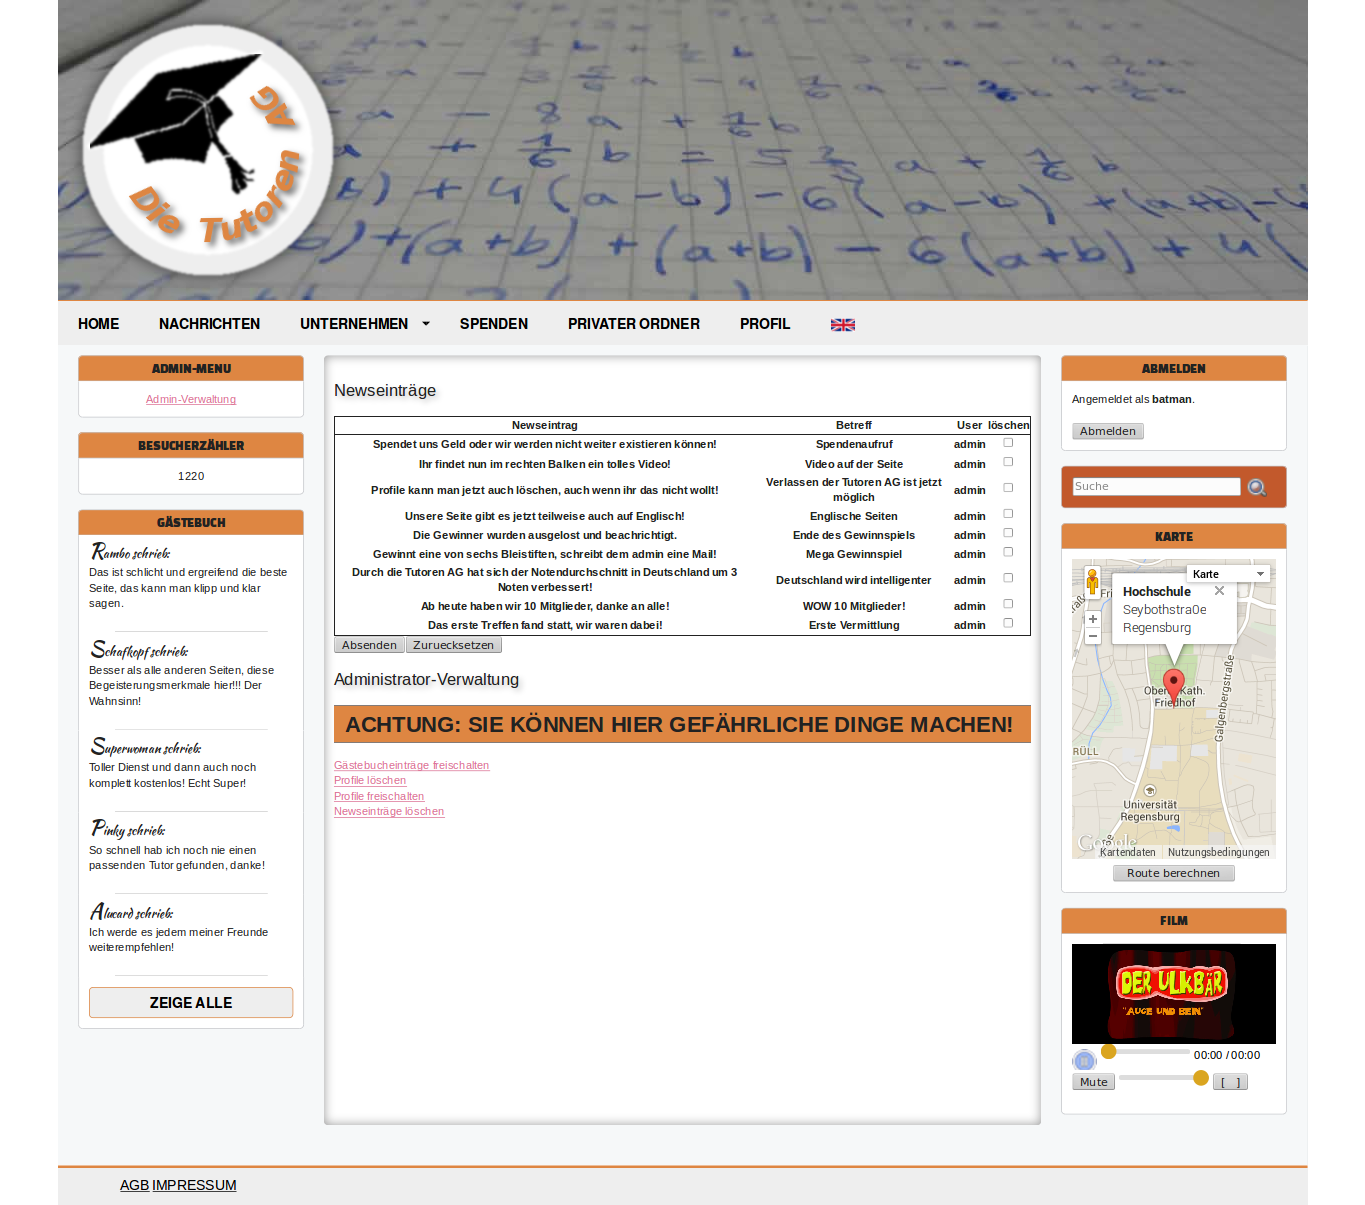
\includegraphics[width=1\textwidth]{../Screenshots/de/admin/admin_news}